%%%%%%%%%%%%%%%%%%%%%%%%%%%%%%%%%
\newpage
%%%%%%%%%%%%%%%%%%%%%%%%%%%%%%%%%
\section{The transition to the Fourier Transform}

\subsection*{Resources}
\begin{itemize}
    \item Book: Chapter 2 (\url{https://see.stanford.edu/materials/lsoftaee261/book-fall-07.pdf})
    \item Video I: Last part of lecture 5 (\url{https://www.youtube.com/watch?v=X5qRpgfQld4})
    \item Video II: First part of lecture 6 (\url{https://www.youtube.com/watch?v=4lcvROAtN_Q})
\end{itemize}

\subsection*{Comment}
Until now we have been considering Fourier series which allows us to describe periodic phenomena. This can however cause issues, such as in challenge \ref{sec:fstexpform} or \ref{sec:nonunitperiods} when the function isn't actually periodic, since the derived fourier series results in periodicity outside the region of integration. The Fourier transform can help overcome this limitation and accurately describe signals which are non-periodic.

The suggested resources provide an excellent intuetive path to the connection between Fourier Series and Fourier Transforms, and this challenge is designed to give you the opportunity to take some time to try to understand the main concepts behind the transition.

\subsection*{Challenge}
Imagine you are writing a letter to a student, explaining about the basis for the Fourier transform. You may assume that the student knows about Fourier series well, but nothing about Fourier transforms. Explain about the transition, including descriptions of the concepts, equations and variables involved. Please use the suggested resources above as a basis for the description, however you may also use additional resources too if you cite them. A length of about 1 side of A4 is suggested, although you may use more if you feel it is necessary. Please write neatly and clearly, since the intention is to share your description with the teacher and other students. You may do this in hand-written or digital form.

\subsection*{Solution}
After completion, please read at least 2 other students' interpretations. The teacher will also review the contents to help ensure sufficient understanding of the concepts, and may publish your description for everyone to learn from (if you want this to be anonymous, please add a note saying this).

\timebox




%%%%%%%%%%%%%%%%%%%%%%%%%%%%%%%%%
\newpage
%%%%%%%%%%%%%%%%%%%%%%%%%%%%%%%%%
\section{Fourier transform notation}

\subsection*{Resources}
\begin{itemize}
    \item Book: Chapter 2 (\url{https://see.stanford.edu/materials/lsoftaee261/book-fall-07.pdf})
    \item Video: Lecture 6 (\url{https://www.youtube.com/watch?v=4lcvROAtN_Q})
\end{itemize}

\subsection*{Challenge}
Add the points of the legitimate forms of Fourier notation:

1 point: $\displaystyle \mathcal{F}f(w)=\frac{1}{\sqrt{2 \pi}} \int_{-\infty}^{\infty} e^{i w t} f(t) dt$

2 points: $\displaystyle \mathcal{F}f(w)=\int_{-\infty}^{\infty} e^{-i 2 \pi w t} f(t) dt$

4 points: $\displaystyle \mathcal{F}f(w)=\frac{1}{2 \pi} \int_{-\infty}^{\infty} e^{i w t} f(t) dt$

8 points: $\displaystyle \mathcal{F}f(s)=\frac{1}{\sqrt{2 \pi}} \int_{-\infty}^{\infty} e^{i \pi s t} f(t) dt$

16 points: $\displaystyle \mathcal{F}f(w)=\int_{-\infty}^{\infty} e^{i 2 \pi w t} f(t) dt$

32 points: $\displaystyle \mathcal{F}f(s)=\int_{-\infty}^{\infty} e^{-i s t} f(t) dt$

\subsection*{Solution}
\hash{eee}{58851c}

\timebox




%%%%%%%%%%%%%%%%%%%%%%%%%%%%%%%%%
\newpage
%%%%%%%%%%%%%%%%%%%%%%%%%%%%%%%%%
\section{L'H\^opital's rule}

\subsection*{Challenge}
Use L'H\^opital's rule to determine the limit of
\begin{equation}
    \frac{Sin(x)}{x}
\end{equation}
as $x \rightarrow 0$.

\subsection*{Solution}
\hash{ccc}{9cc92f}

\timebox




%%%%%%%%%%%%%%%%%%%%%%%%%%%%%%%%%
\newpage
%%%%%%%%%%%%%%%%%%%%%%%%%%%%%%%%%
\section{Fourier transform of a window function}
\label{sec:tophat}

\subsection*{Resources}
\begin{itemize}
    \item Book: Chapter 2 (\url{https://see.stanford.edu/materials/lsoftaee261/book-fall-07.pdf})
    \item Video: Lecture 6 (\url{https://www.youtube.com/watch?v=4lcvROAtN_Q})
\end{itemize}

\subsection*{Comments}
This challenge, and the next few, represent very common functions that can be evaluated using the Fourier transform. Try to understand the mathematics used in their evaluation.

\subsection*{Challenge}
Calculate the Fourier Transform for the window function

\begin{equation}
    f(t)=
    \begin{cases}
        1 & \text{for } |t| < 1/2 \\
        0 & \text{for } |t| > 1/2
    \end{cases}
\end{equation}

In graph-form the function and its transform appear as follows:

\begin{tabular}{cc}
    \textbf{Function} & \textbf{Fourier transform} \\
    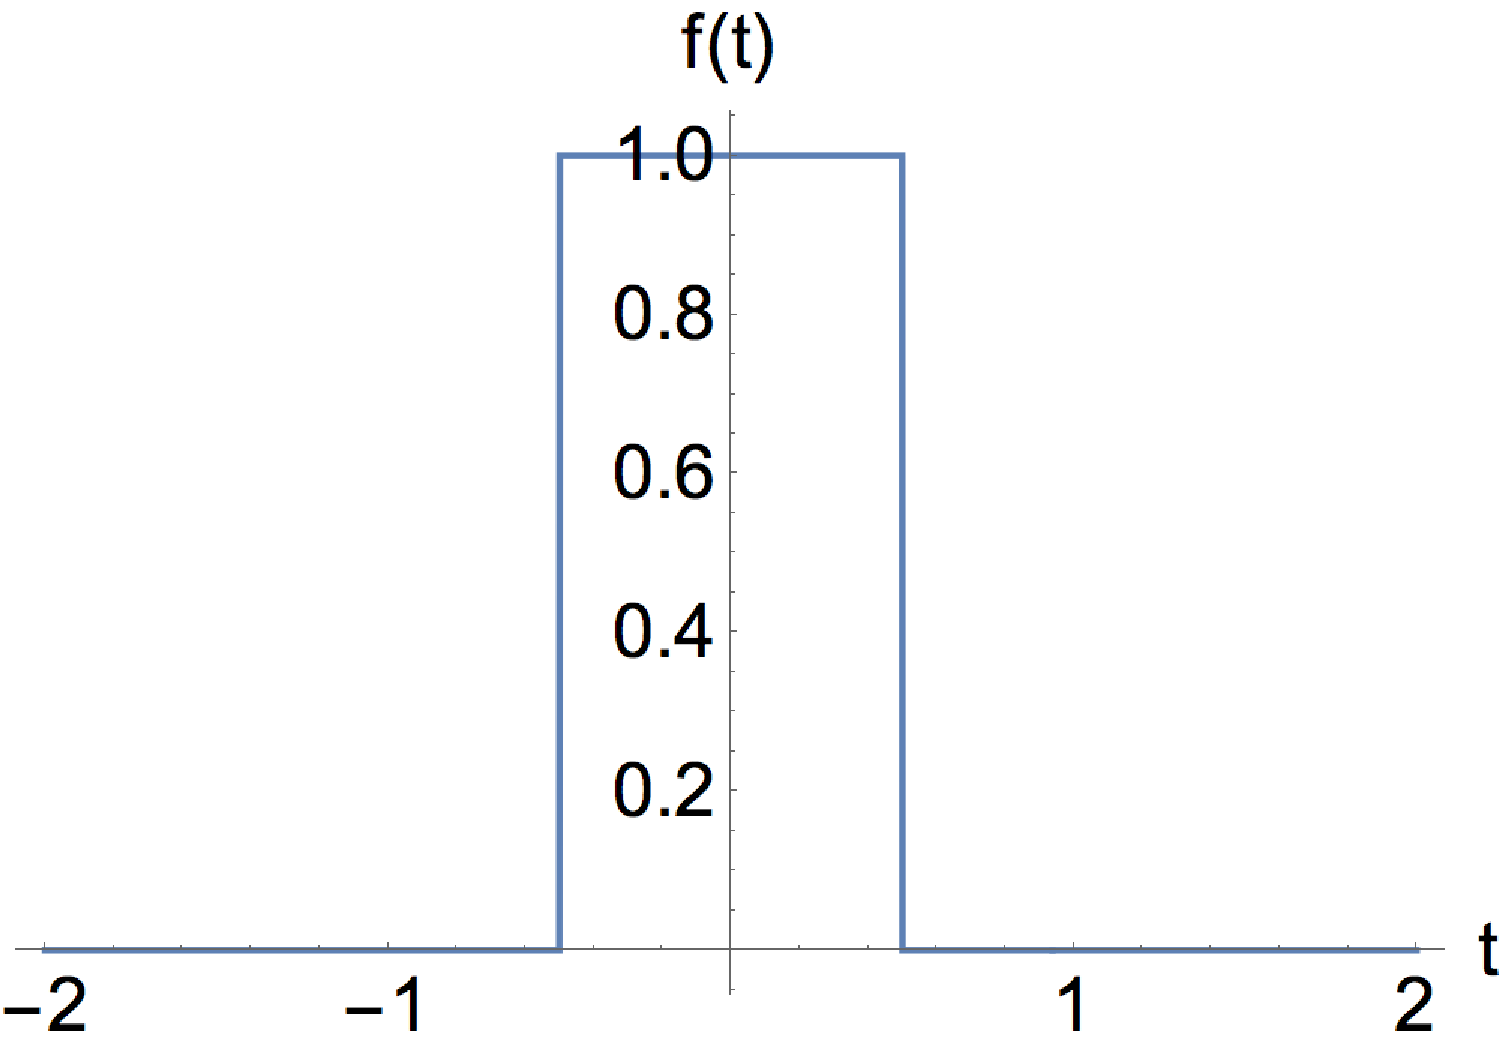
\includegraphics[scale=0.5]{window1.png} & 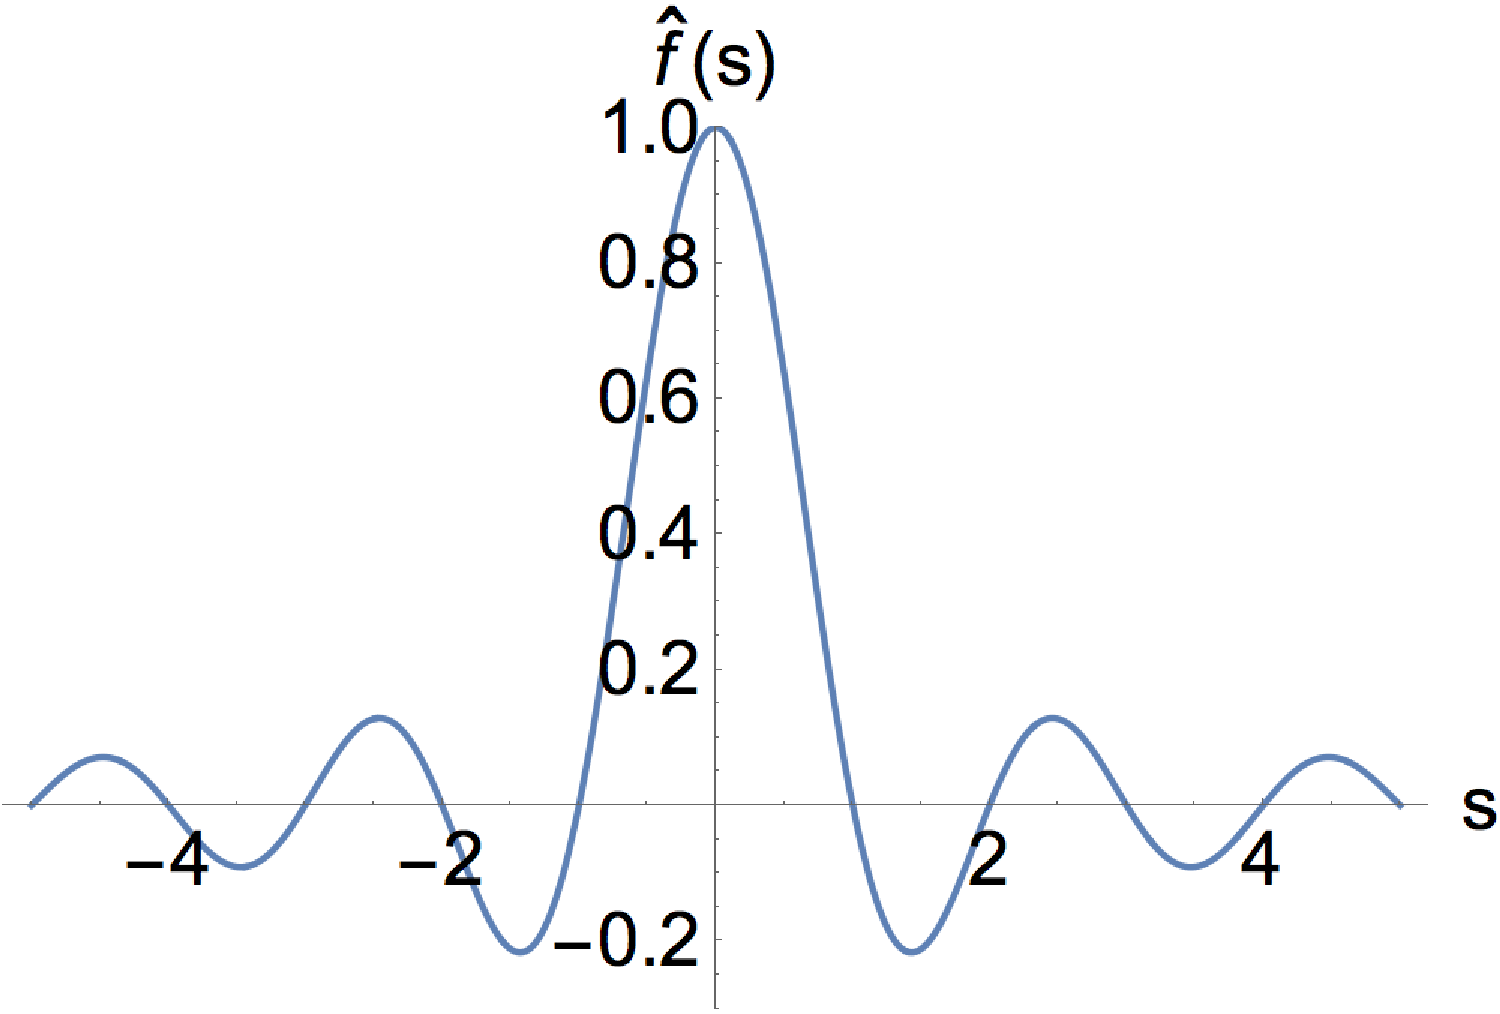
\includegraphics[scale=0.5]{window1ft.png}
\end{tabular}

To check your answer, calculate $\hat{f}(s=1.5)$.

\subsection*{Solution}
\hash{ddd}{b78cd8}

\timebox




%%%%%%%%%%%%%%%%%%%%%%%%%%%%%%%%%
\newpage
%%%%%%%%%%%%%%%%%%%%%%%%%%%%%%%%%
\section{Fourier transform of a triangle function}

\subsection*{Resources}
\begin{itemize}
    \item Book: Chapter 2 (\url{https://see.stanford.edu/materials/lsoftaee261/book-fall-07.pdf})
    \item Video: Lecture 6 (\url{https://www.youtube.com/watch?v=4lcvROAtN_Q})
\end{itemize}

\subsection*{Challenge}
Calculate the Fourier Transform for the triangle function shown below. In graph-form the function and its transform appear as follows:

\begin{tabular}{cc}
    \textbf{Function} & \textbf{Fourier transform} \\
    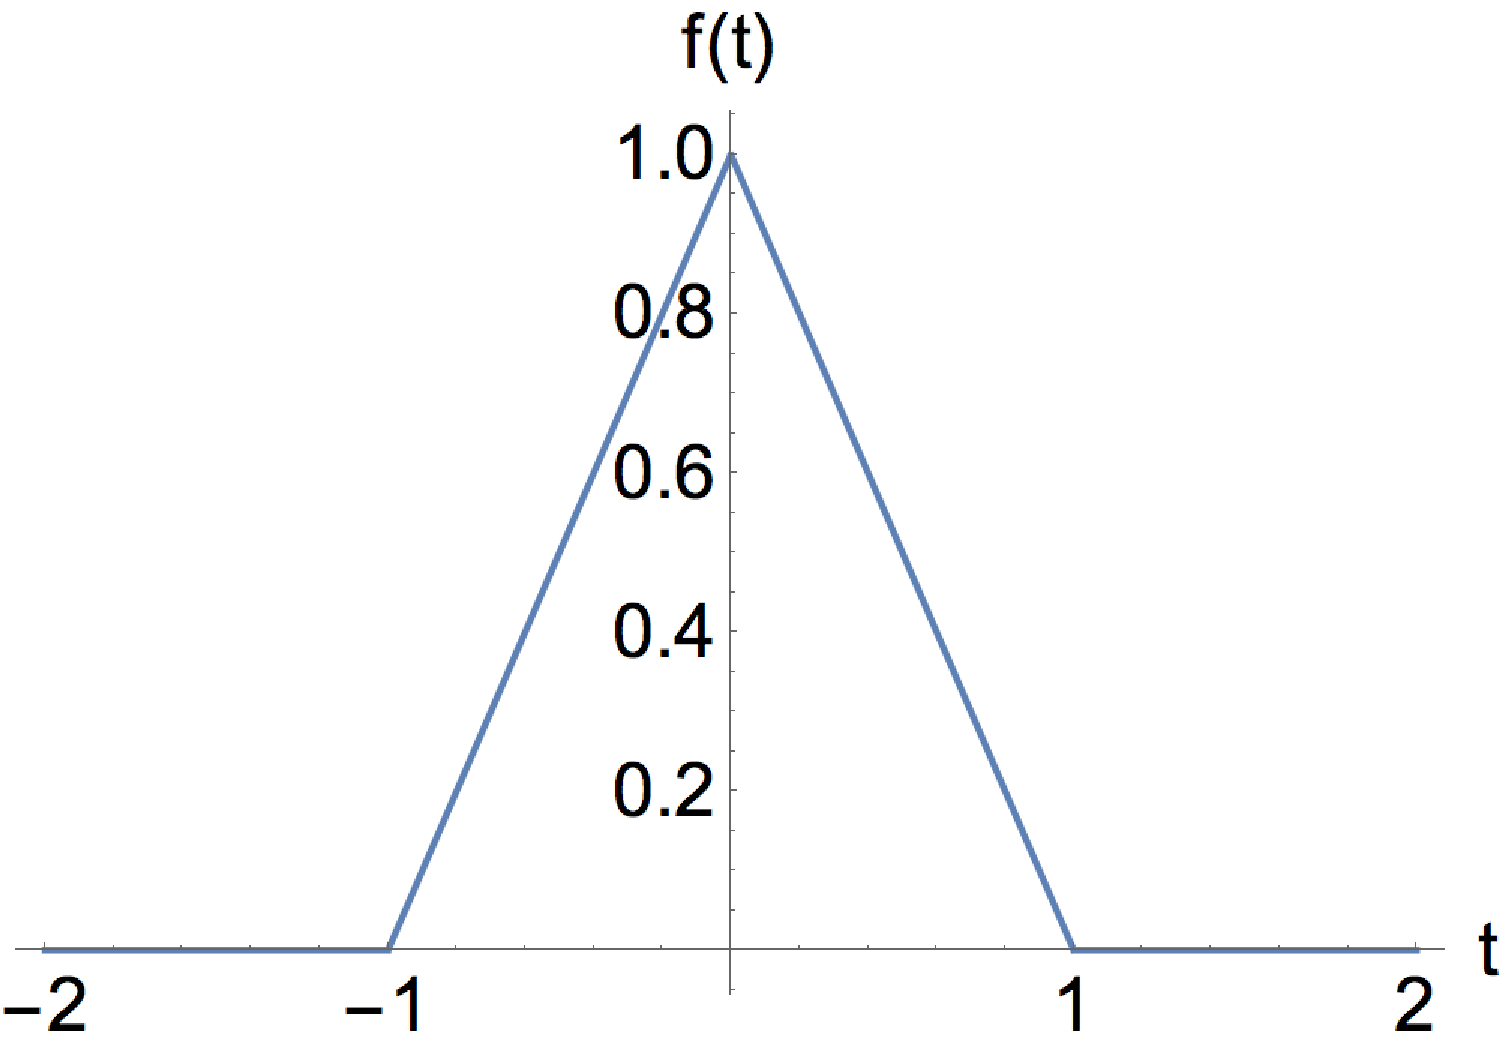
\includegraphics[scale=0.5]{triangle.png} & 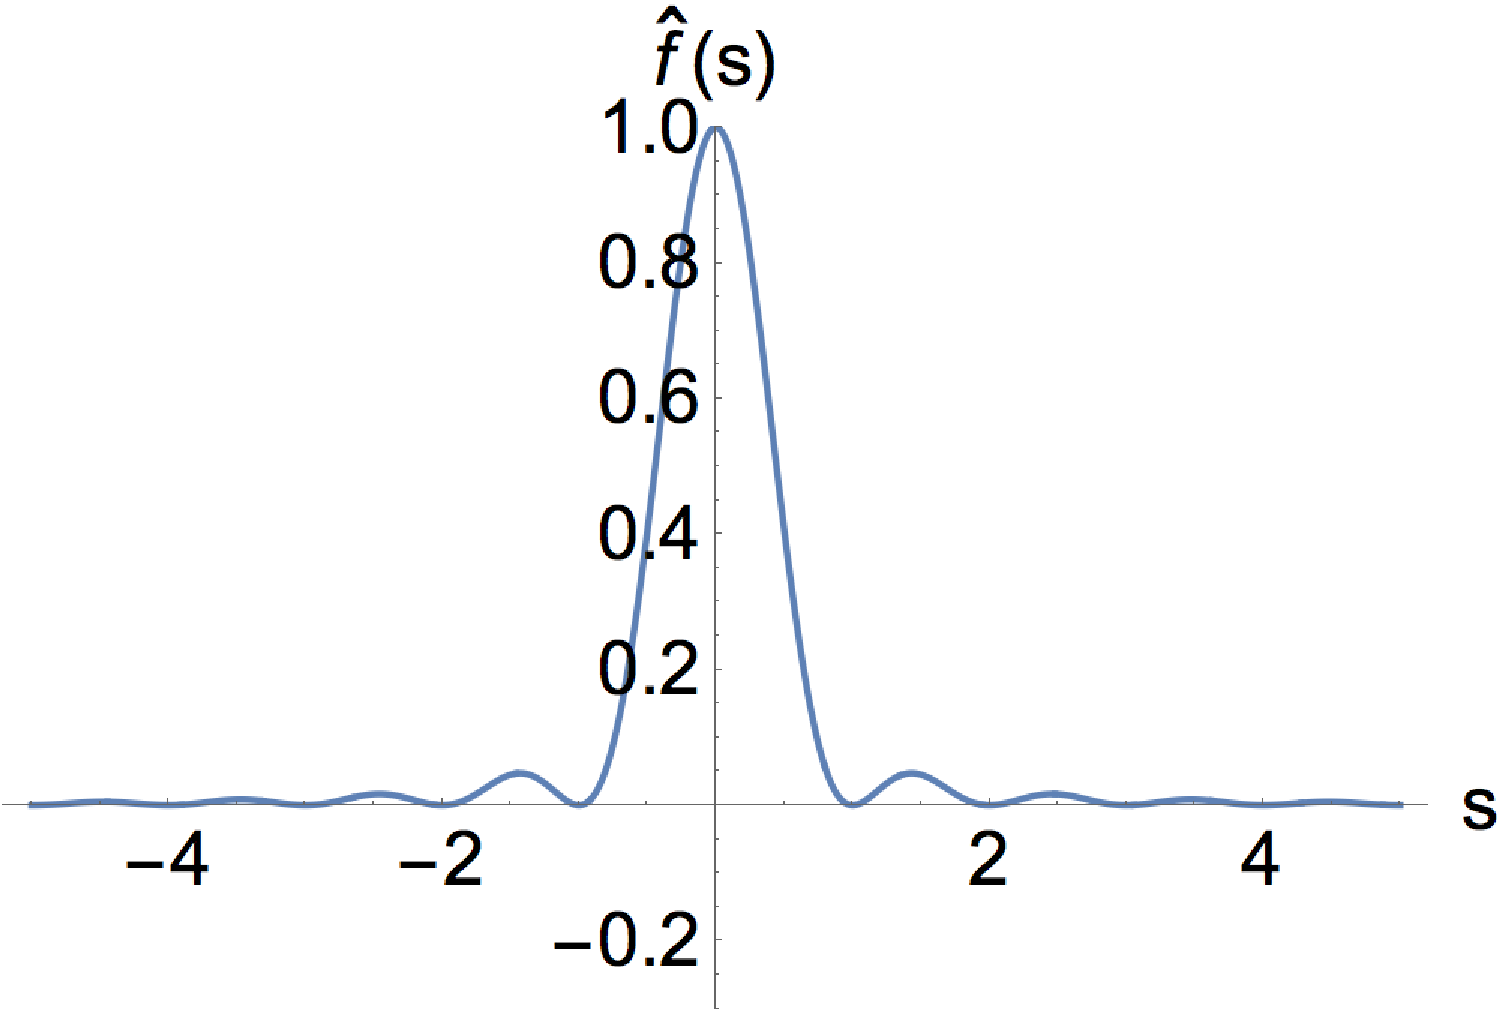
\includegraphics[scale=0.5]{triangleft.png}
\end{tabular}

To check your answer, calculate $\hat{f}(s=1.5)$.

\subsection*{Solution}
\hash{fff}{55e1c1}

\timebox




%%%%%%%%%%%%%%%%%%%%%%%%%%%%%%%%%
\newpage
%%%%%%%%%%%%%%%%%%%%%%%%%%%%%%%%%
\section{Fourier transform of a gaussian}

\subsection*{Resources}
\begin{itemize}
    \item Book: Chapter 2 (\url{https://see.stanford.edu/materials/lsoftaee261/book-fall-07.pdf})
    \item Video: Lecture 7 (\url{https://www.youtube.com/watch?v=mdFETbe1n5Q})
\end{itemize}

\subsection*{Challenge}
Calculate the Fourier Transform for the gaussian function:

\begin{equation}
    f(t) = e^{-\pi t^2}
\end{equation}

The gaussian function looks like

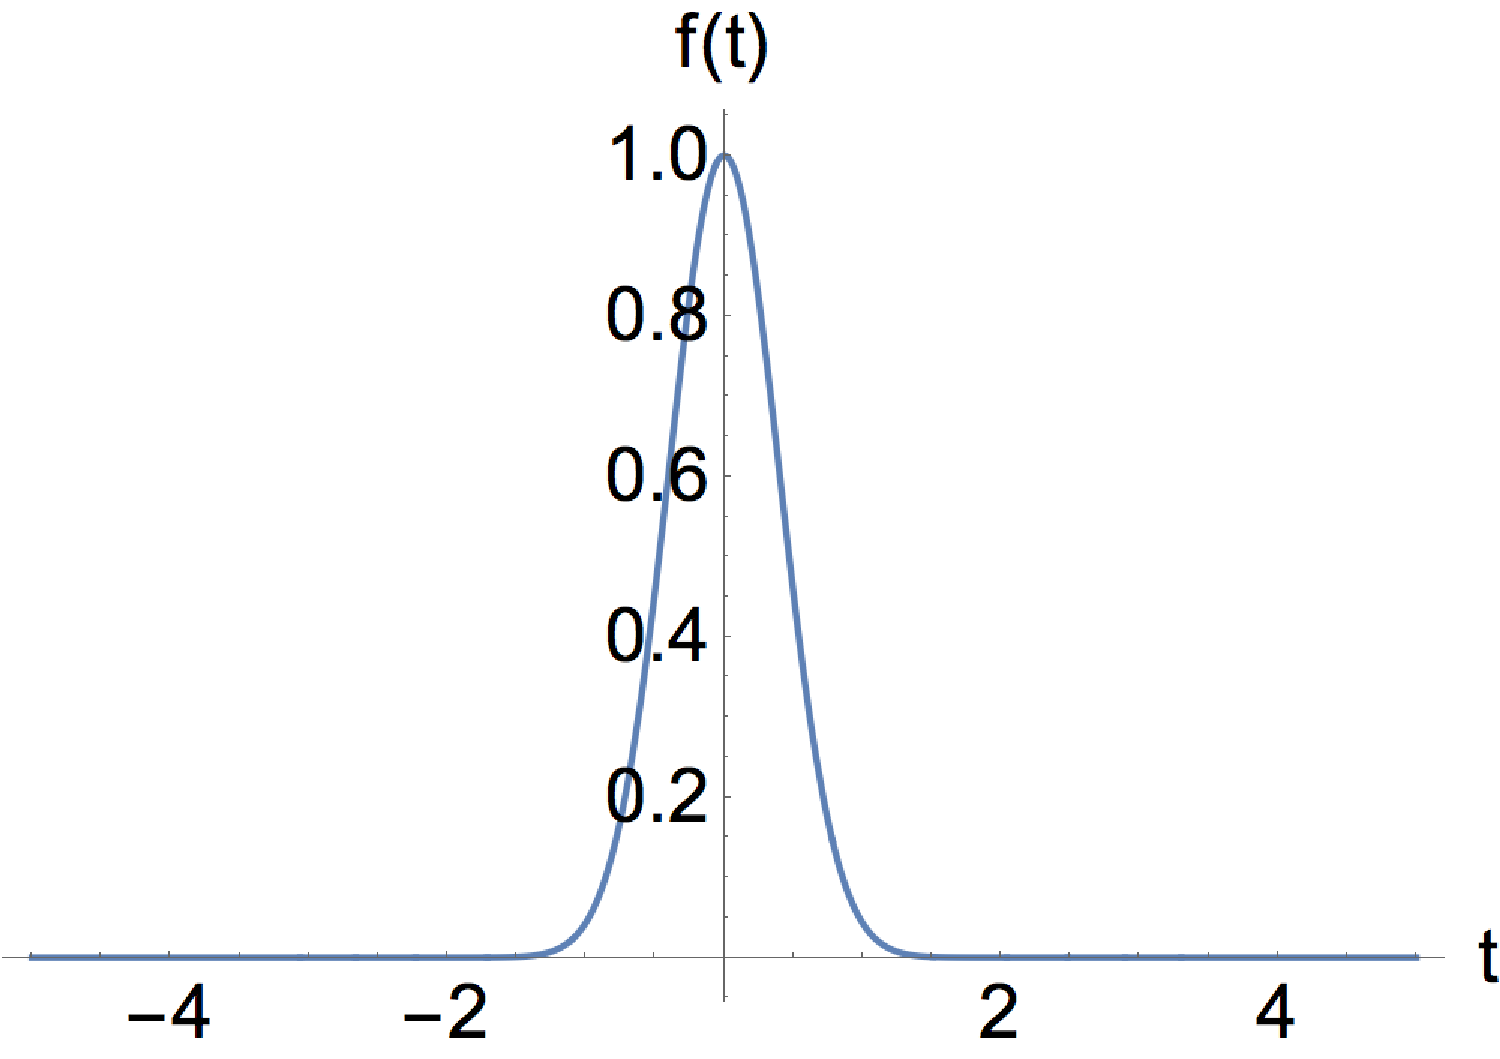
\includegraphics{gaussian.png}

To check your answer, calculate $\hat{f}(s=1.5)$.

\subsection*{Solution}
\hash{ggg}{341b23}

\timebox




%%%%%%%%%%%%%%%%%%%%%%%%%%%%%%%%%
\newpage
%%%%%%%%%%%%%%%%%%%%%%%%%%%%%%%%%
\section{Fourier transform of a rocket function}

\subsection*{Resources}
\begin{itemize}
    \item Book: Chapter 2.2.6 (\url{https://see.stanford.edu/materials/lsoftaee261/book-fall-07.pdf})
\end{itemize}

\subsection*{Challenge}
Calculate the Fourier Transform for the rocket function shown below. In graph-form the function and its transform appear as follows:

\begin{tabular}{cc}
    \textbf{Function} & \textbf{Fourier transform} \\
    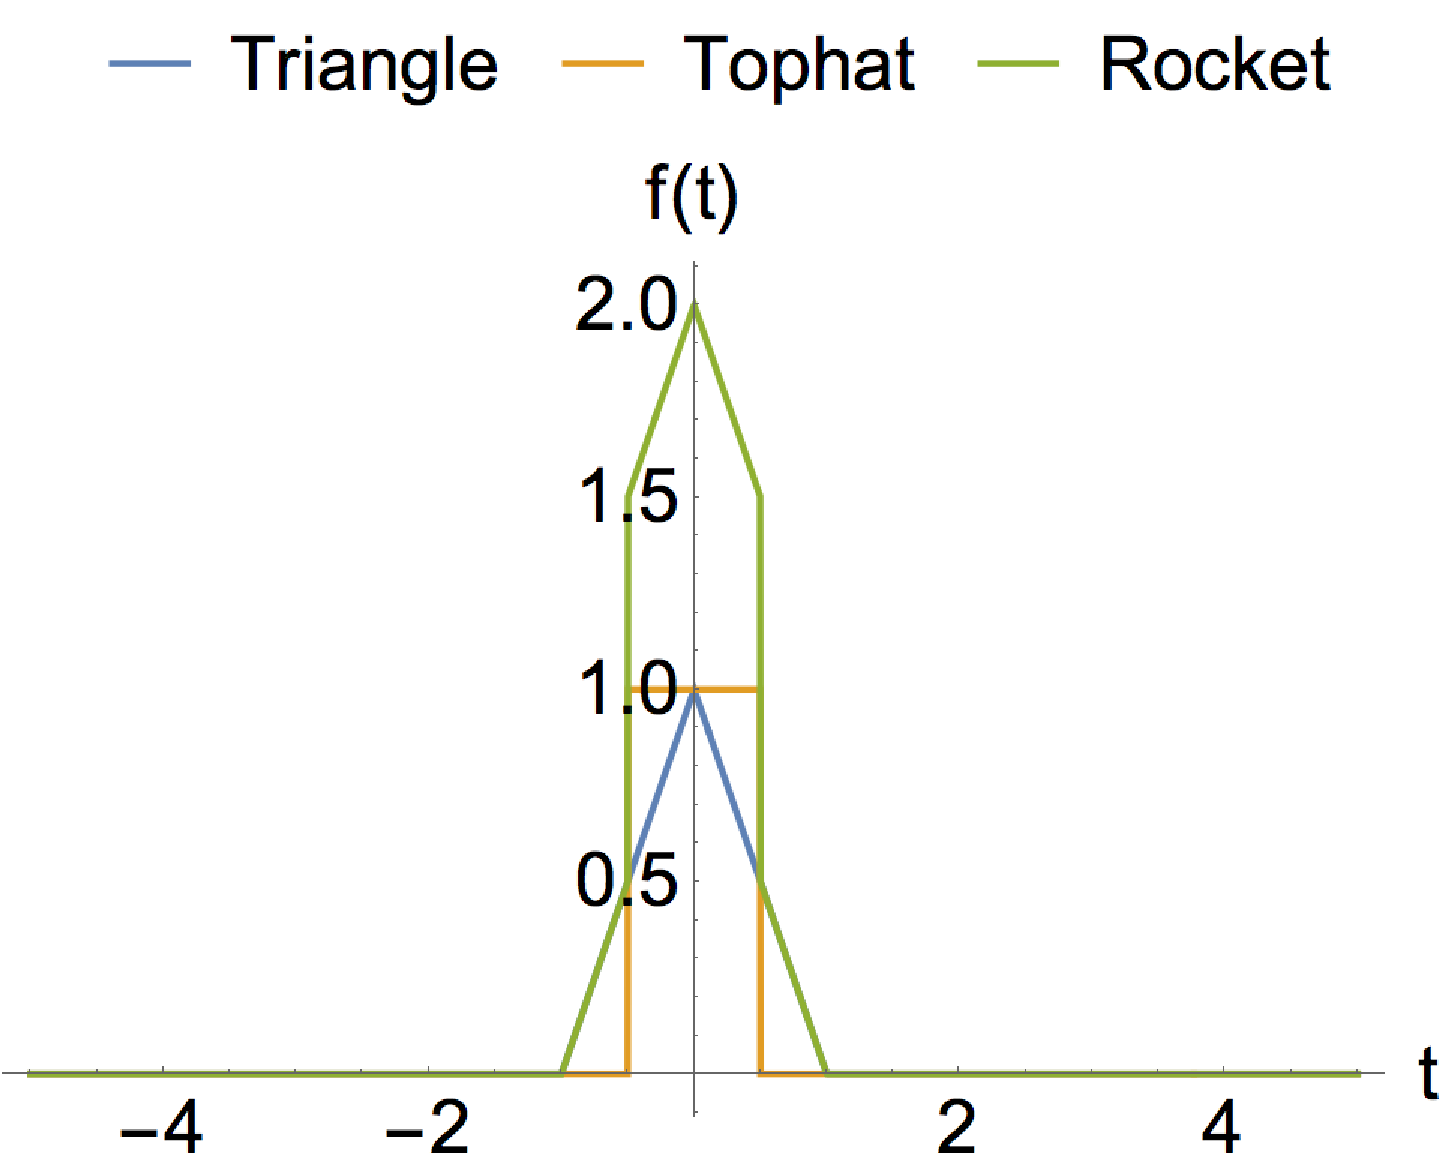
\includegraphics[scale=0.5]{rocket.png} & 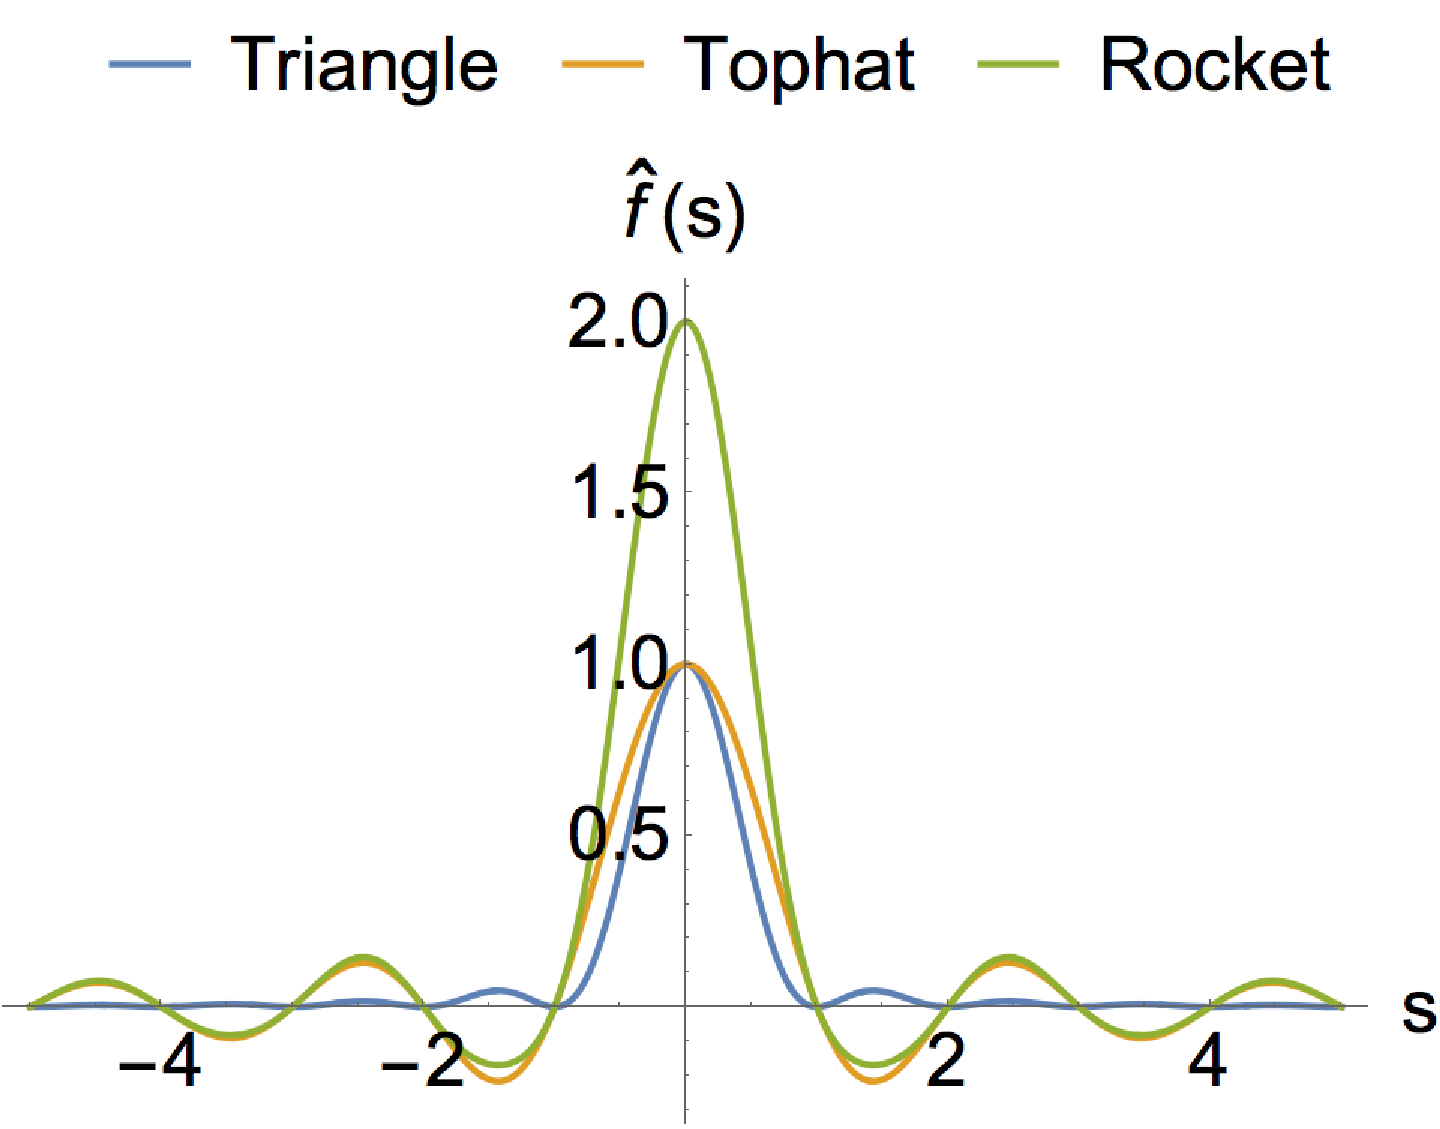
\includegraphics[scale=0.5]{rocketft.png}
\end{tabular}

To check your answer, calculate $\hat{f}(s=1.5)$.

\subsection*{Solution}
\hash{hhh}{a344fd}

\timebox




%%%%%%%%%%%%%%%%%%%%%%%%%%%%%%%%%
\newpage
%%%%%%%%%%%%%%%%%%%%%%%%%%%%%%%%%
\section{Fourier transform of a shifted window function}

\subsection*{Resources}
\begin{itemize}
    \item Book: Chapter 2.2.7 (\url{https://see.stanford.edu/materials/lsoftaee261/book-fall-07.pdf})
\end{itemize}

\subsection*{Challenge}
1. By delaying the window function slightly as shown below, we are introducing a phase-shift. Write a few sentences explaining what is meant by a phase-shift and how it relates to the current situation.

2. Calculate the Fourier Transform for the window function delayed by $1/100$ s, $1/10$ s and $1$ s.

3. Write a short summary of how the real and imaginary parts of the signal are changing as the delay increases. You considered the original window function in challenge \ref{sec:tophat}.

\begin{tabular}{c}
    \textbf{Function} \\
    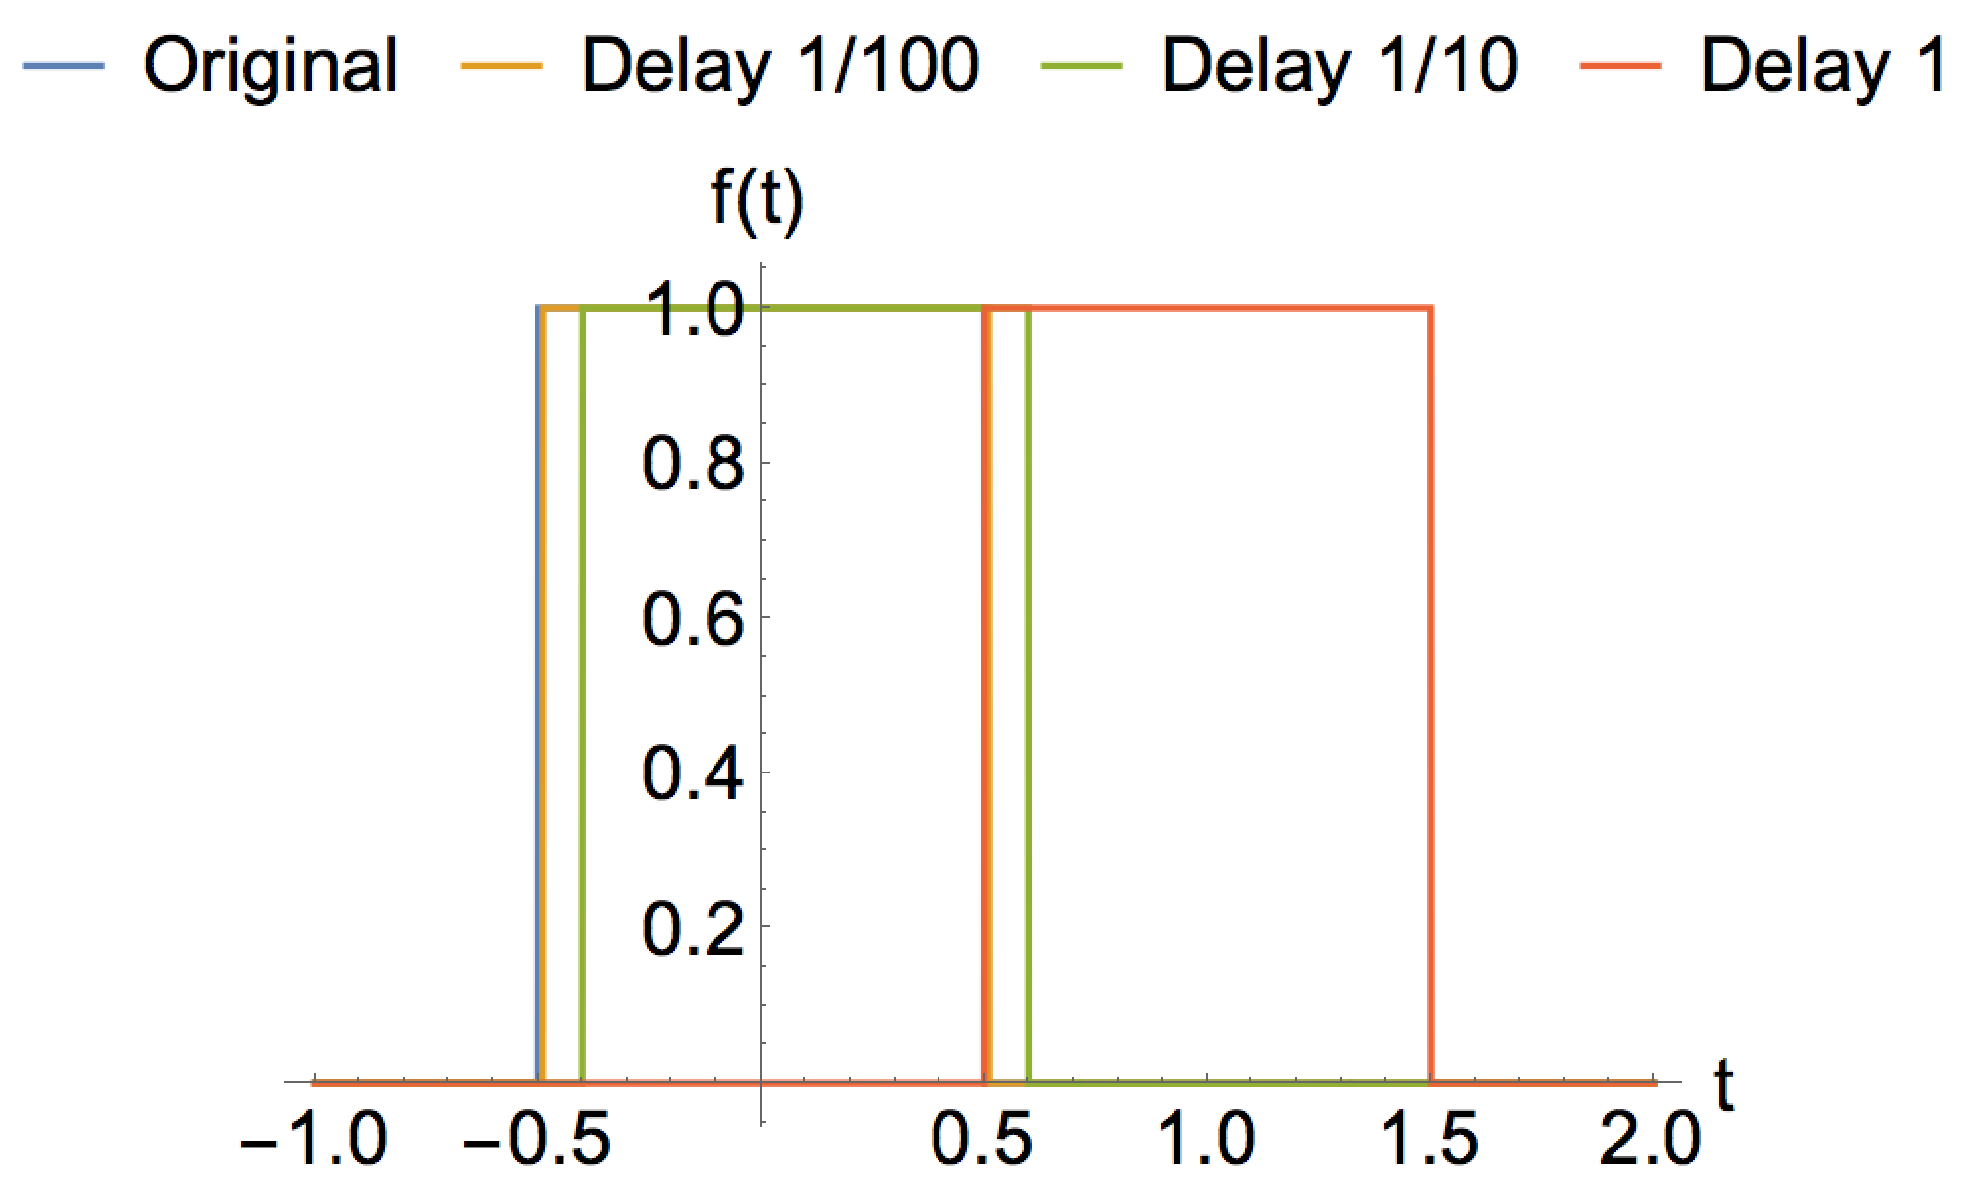
\includegraphics[scale=0.5]{tophatdelay.png}
\end{tabular}

\begin{tabular}{cc}
    \textbf{Fourier transform (real part)} & \textbf{Fourier transform (imaginary part)}\\
    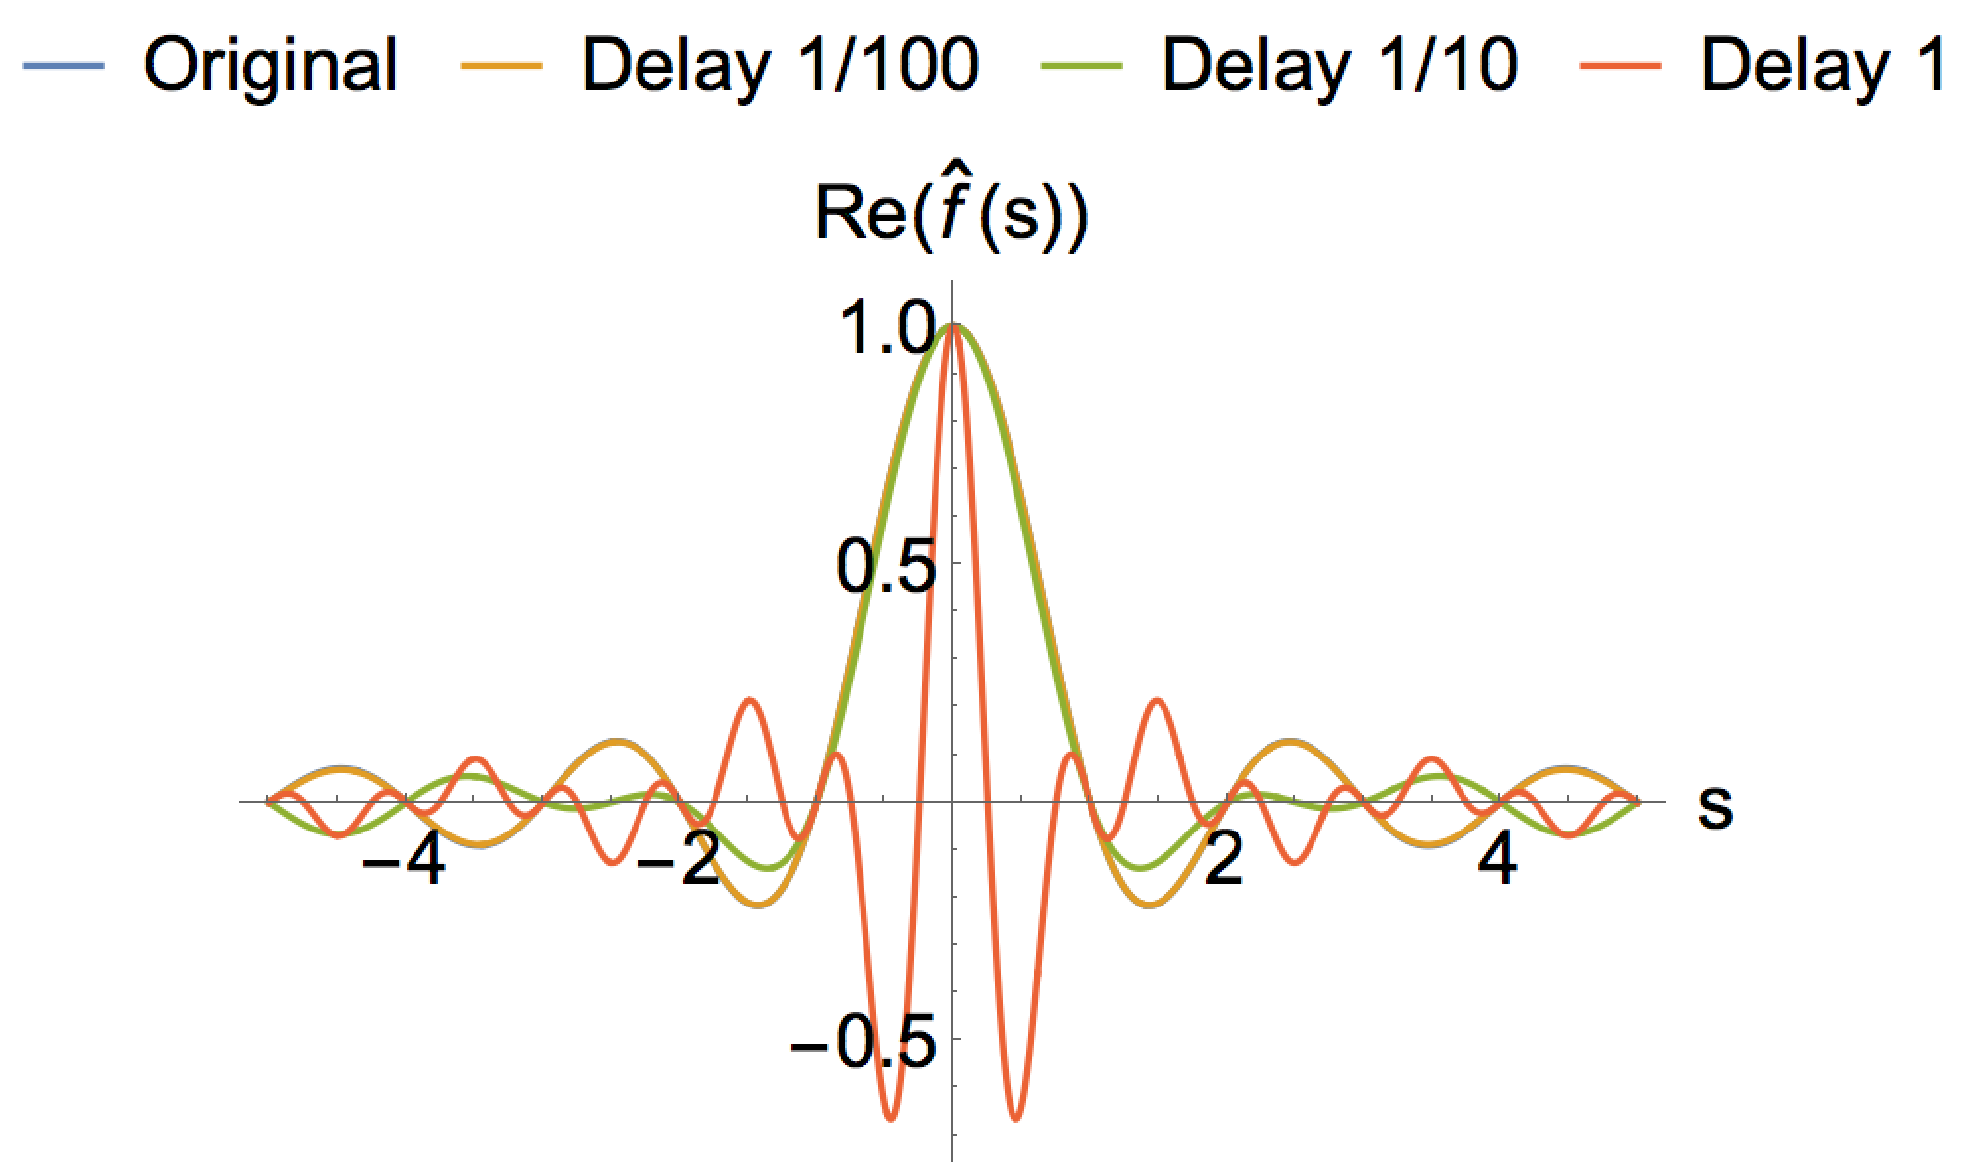
\includegraphics[scale=0.5]{tophatdelayre.png} & 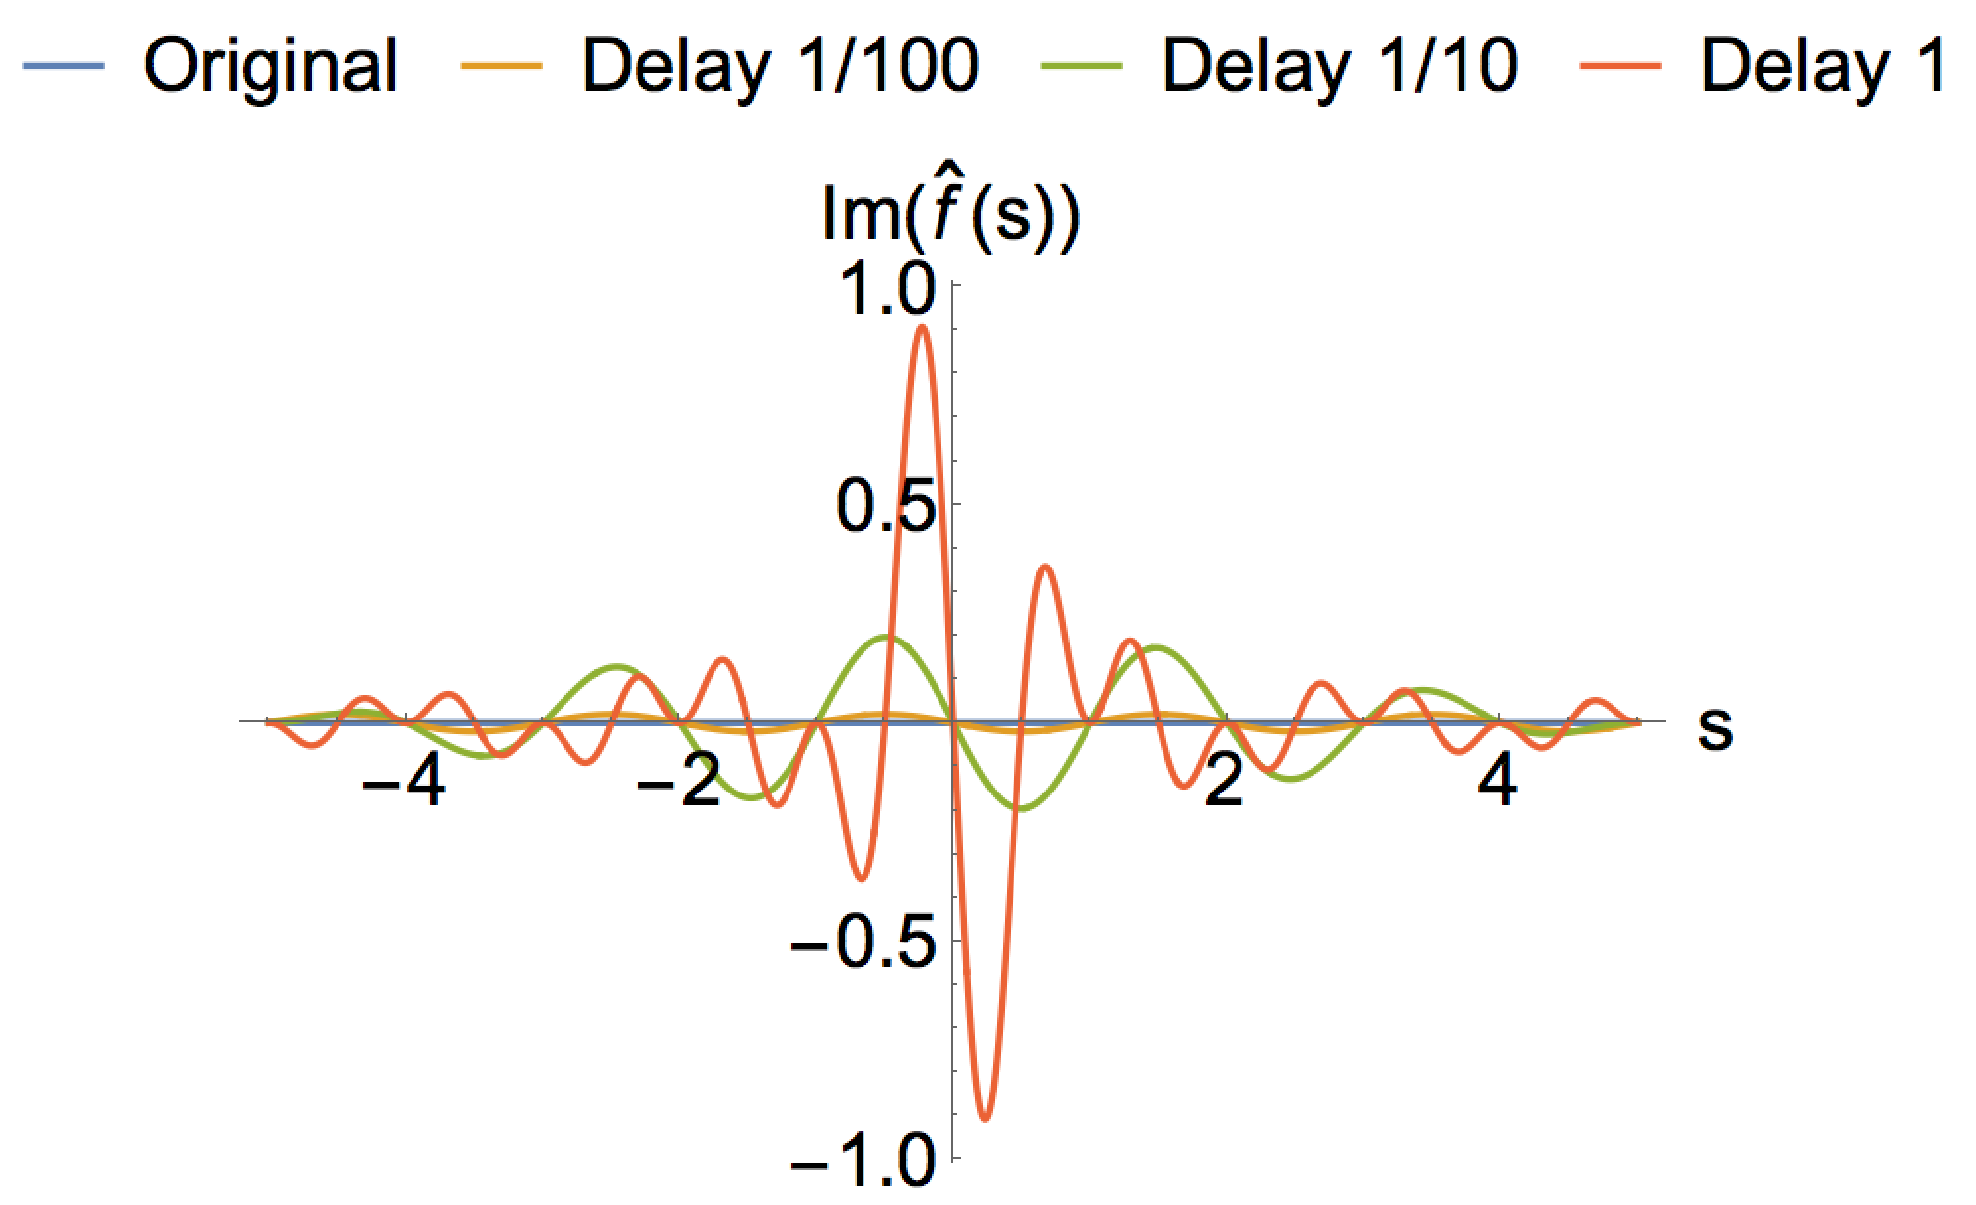
\includegraphics[scale=0.5]{tophatdelayim.png}
\end{tabular}

To check your answer, calculate $\hat{f}(s=2.9)$ for each case. By doing this, you will also gain insight into the new nature of the real and imaginary parts of the function with shifting.

\subsection*{Solution}
$1/100$ s delay: $0.0333568 - 0.0061462i$

$1/10$ s delay: $-0.00843515 - 0.0328527i$

$1$ s delay: $0.0274405 + 0.0199367i$

\timebox


% Need to do an exmaple with fourier transform (square wave?) Is in in the PDF? https://www.youtube.com/watch?annotation_id=annotation_655167&feature=iv&src_vid=8JKb9UN6W4c&v=_HJH3MekMHY

% Next: continue to figure out what the fourier transform is, and try to make a problem with it.

% 2.2.4 pairs and duality?
% 2.2.6: Linearity, shift, stretch


% Show that Sin(x)/x is 1 at x=0

% Calculate fourier transform of dirichlet window https://www.youtube.com/watch?annotation_id=annotation_655167&feature=iv&src_vid=8JKb9UN6W4c&v=_HJH3MekMHY
